% Possíveis TODO
% - expandir nas equacoes xx yy
\documentclass[a4paper,titlepage]{article}
\usepackage[utf8]{inputenc}
\usepackage[T1]{fontenc}
\usepackage[portuges]{babel}
% setspace - \doublespace \onehalfspace
% fullpage - ??
\usepackage{verbatim}
\usepackage{url}
\usepackage{hyperref}
\usepackage{graphicx}
\usepackage[bf]{subfigure}
\usepackage[bf]{caption}
\usepackage{amsmath,amssymb}
\usepackage{algorithm,algorithmic}
\usepackage{mathtools,empheq}
\usepackage{macrosfabbri-basic}
\usepackage{xcolor}

% ------------------------------------------------------------------------------
% Paper draft Comments and TODO's
%
% You have two versions of the macro
% \draftnote{My note}. The first version puts notes (e.g. My note in the example)
% into the margin of your document. The second formats the note as nothing. You
% 'comment out' the version of the macro you don't want (using a % at the
% beginning of the line).
\newcommand{\draftnote}[1]{\marginpar{\tiny\raggedright\textsf{\textcolor{blue}{\hspace{0pt}#1}}}}
%\newcommand{\draftnote}[1]{}
%
% This one is just for the comments for in-line text.
\newcommand{\indraftnote}[1]{\textcolor{blue}{\texttt{\footnotesize [#1]}}}
\newcommand{\todo}[1]{\indraftnote{todo: #1}} % Este  "a fazer" é para eu não esquecer



\begin{document}

\begin{titlepage}
\renewcommand{\title}{%
  {\LARGE Revis�o Comentada de Artigo}\\
  \mbox{Barycentric Subspace Analysis on Manifolds}%
}
\renewcommand{\author}{Nome Sobrenome}
\renewcommand{\date}{\today}
\newcommand{\info}{%
  \raisebox{4pt}[-4pt]{%
  
\includegraphics[height=1.3cm]{figs/logo-iprj.png} 
  \hspace{0.1in}
  }\\

  Instituto Polit�cnico -- IPRJ\\
  Universidade do Estado do Rio de Janeiro\\[2em]
  
  
\includegraphics[height=1.3cm]{figs/logo-ppgmc.png}\\
  Programa de P�s Gradua��o em Modelagem Computacional\\
  Disciplina de Variedades Diferenci�veis\\
  prof. Ricardo Fabbri\\[1em]

  Nova Friburgo, \date\\[1.5cm]
}

%% Abstand zwischen oberem Blattrand und Titel.
\newlength{\topToTitle} 
\setlength{\topToTitle}{0pt}

%% Abstand zwischen linkem Blattrand und Titel.
\newlength{\leftToTitle} 
\setlength{\leftToTitle}{-60pt}

%% Abstand zwischen Titel und Info-Feld.
\newlength{\titleToInfo} 
\setlength{\titleToInfo}{10cm}

%% \myTextWidth erhoehen, um Info-Feld weiter nach Rechts zu schieben.
\newlength{\myTextWidth}
\setlength{\myTextWidth}{\textwidth}
\advance\myTextWidth by 1cm


\thispagestyle{empty}
\vspace*{\topToTitle}
\begin{minipage}{\myTextWidth}
  \sffamily
  \hspace*{\leftToTitle}\begin{minipage}{11cm}
    \Large\textbf{Trabalho final}\\[1.5cm]
    \title\\[1.5cm]
    \author
  \end{minipage}\\

  %% \enlargethispage{} um ggfs. Titel und Info-Feld weiter
  %% auseinanderziehen zu koennen.
  \vspace*{\titleToInfo}

  \begin{minipage}{\textwidth}
    \flushright
    \info
  \end{minipage}
\end{minipage}%
\end{titlepage}


\section{Preliminares}

Este trabalho consiste em expandir o artigo de Paolo Zaini~\textit{et~al.}
intitulado ''\textit{Parameters estimate of Riemannian Gaussian distribution in
the manifold of covariance matrices.}``~\cite{zanini:hal-01325055},
cuja primeira página está reproduzida na Figura~\ref{fig:paper:page1}.
O presente texto é uma versão comentada do artigo,
expandindo o máximo possível os conceitos ligados a Variedades Diferenciáveis.
Desta forma, o presente texto é um superconjunto do referido artigo.
Ele contém todo o artigo, possivelmente em forma de recortes, com expansões e
comentários, e conexões com outros conceitos.

\begin{figure}
\centering
\frame{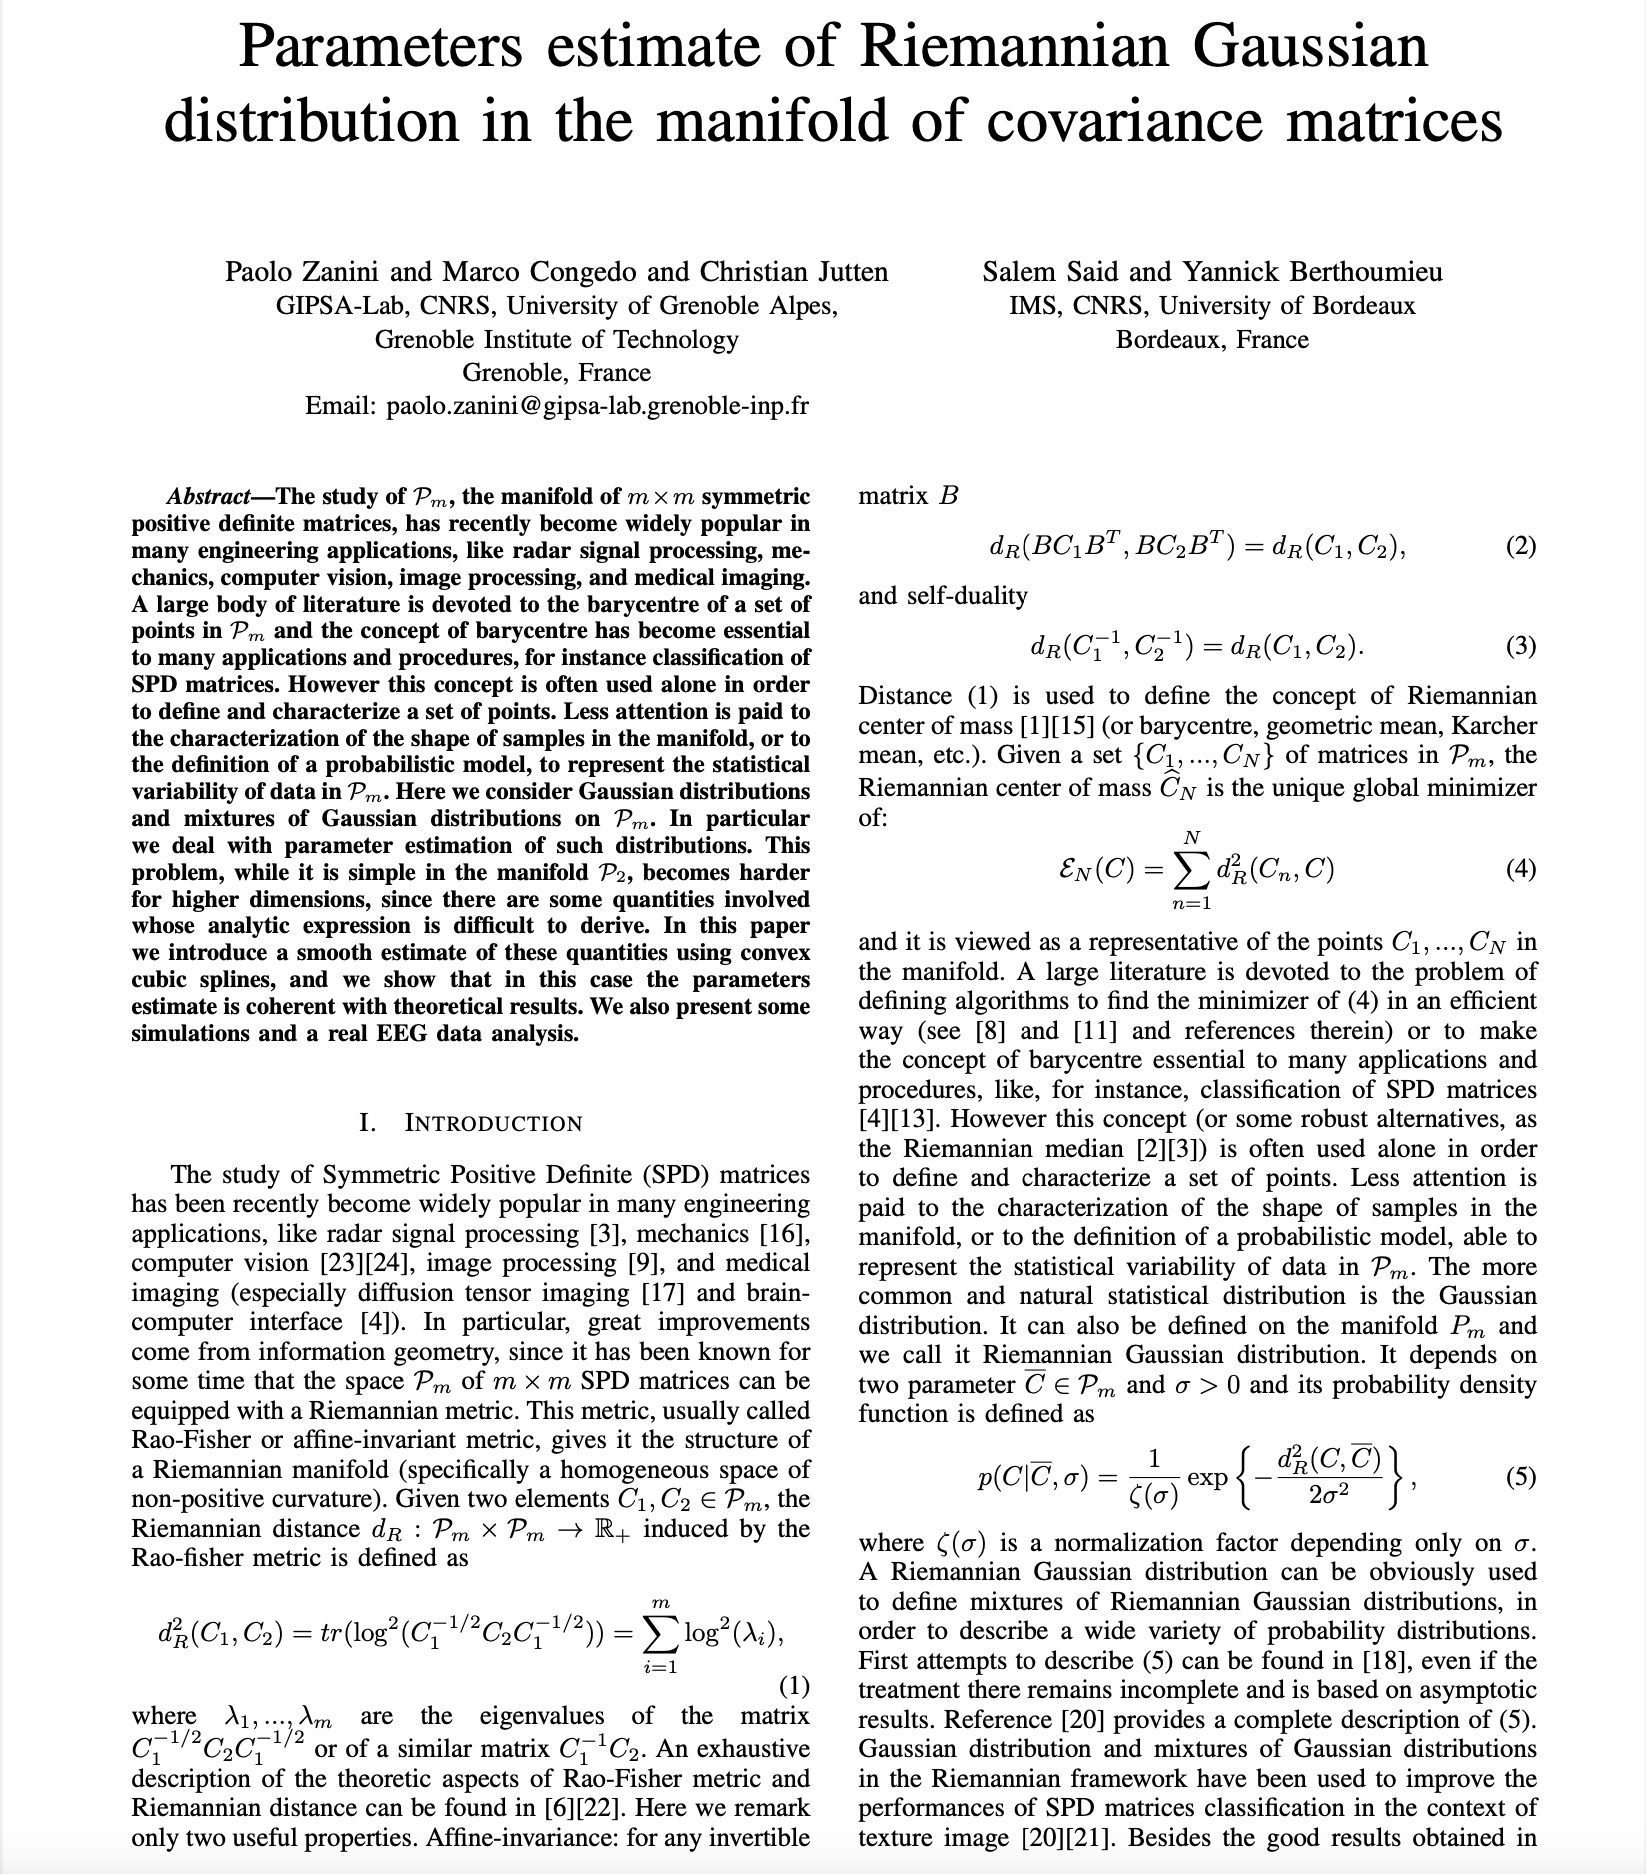
\includegraphics[width=.9\linewidth]{figs/page-01.png}}
\caption{% 
Primeira página do artigo sendo revisado. Acessível pela URL
\url{https://hal.inria.fr/hal-01325055}.
}\label{fig:paper:page1}
\end{figure}

Será utilizada uma mistura de línguas nesta revisão, sendo o inglês preferido
sempre que possível. Sendo assim, não teremos o trabalho de traduzir do inglês
algumas construções básicas do \LaTeX\ como \emph{Theorem} ou
\emph{Definition}.


\section{Tabela de Notação}

This section has a summary of the notation used in the paper.

\section{Commented and Expanded Abstract}

A figura a seguir mostra o \textit{Abstract} do paper. Os autores abordam o
estudo da variedade $\mathcal{P}_m$ das matrizes simétricas positivas-definidas
de dimensão $m \times m$. Este campo de pesquisa ultimamente tem se tornado
amplamente empregado em várias áreas da engenharia, como processamento de
sinais, visão computacional, processamento de imagens, valendo destacar a área
de imagiologia médica. Esta última é uma especialidade médica que se ocupa do
uso das tecnologias de imagem para realização de diagnósticos. As análises
realizadas neste trabalho utilizam dados simulados e dados reais de
Eletroencefalografia ou EEG, que é um método de monitoramento eletrofisiológico
utilizado para registrar a atividade elétrica do cérebro. 

\begin{center}
  \vspace{1em}
  \frame{\centering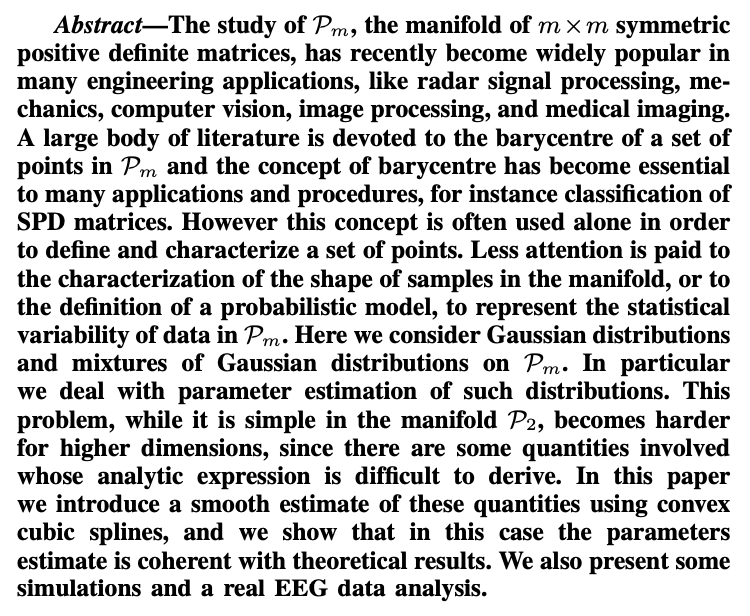
\includegraphics[width=0.8\linewidth]{figs/abstract.png}}
  \vspace{1em}
\end{center}


No contexto de álgebra linear, uma matriz positiva-definida (SPD, da sigla em
inglês \textit{Symmetric Positive Definite}) é análoga a um número real
positivo em muitos aspectos. Uma matriz simétrica $M$ com entradas reais é
positiva-definida se o número real $z^T M z$ é positivo para cada vetor coluna
real não-nulo $z$, onde $z^T$ é o seu
transposto~\cite{doi:PositiveDefiniteMatrices}.  Esta definição ainda pode ser
estendida para o domínio dos números complexos, no caso de matrizes
Hermitianas.

Os autores citam que grande parte da literatura está focada no estudo do
baricentro, ou centro de massa riemanniano, de um conjunto de pontos na
variedade de matrizes simétricas positivas-definidas $\mathcal{P}_m$.  O
conceito de baricentro é de notável importância para muitas aplicações, como a
classificação de SPD's. O problema do centro de massa riemanniano também é
conhecido na literatura como \textit{média riemanniana de
tensores}~\cite{moakher2005differential}.

Entretanto, os autores indagam que o conceito de baricentro tipicamente tem
sido utilizado apenas para a caracterização do conjunto de pontos. Não
obstante, pouca atenção tem sido empregada na caracterização da forma das
amostras na própria variedade ou ainda na definição do modelo probabilístico
que representa e governa a variabilidade estatística dos dados em
$\mathcal{P}_m$.

Neste trabalho, portanto, o problema de estimação de parâmetros de
distribuições Gaussianas em $\mathcal{P}_m$ será explorado para altas
dimensões, onde a tratabilidade do problema é mais difícil comparada ao caso
bidimensional.

\section{Commented and Expanded Section 1: Introduction}

\begin{center}
  \vspace{1em}
  \frame{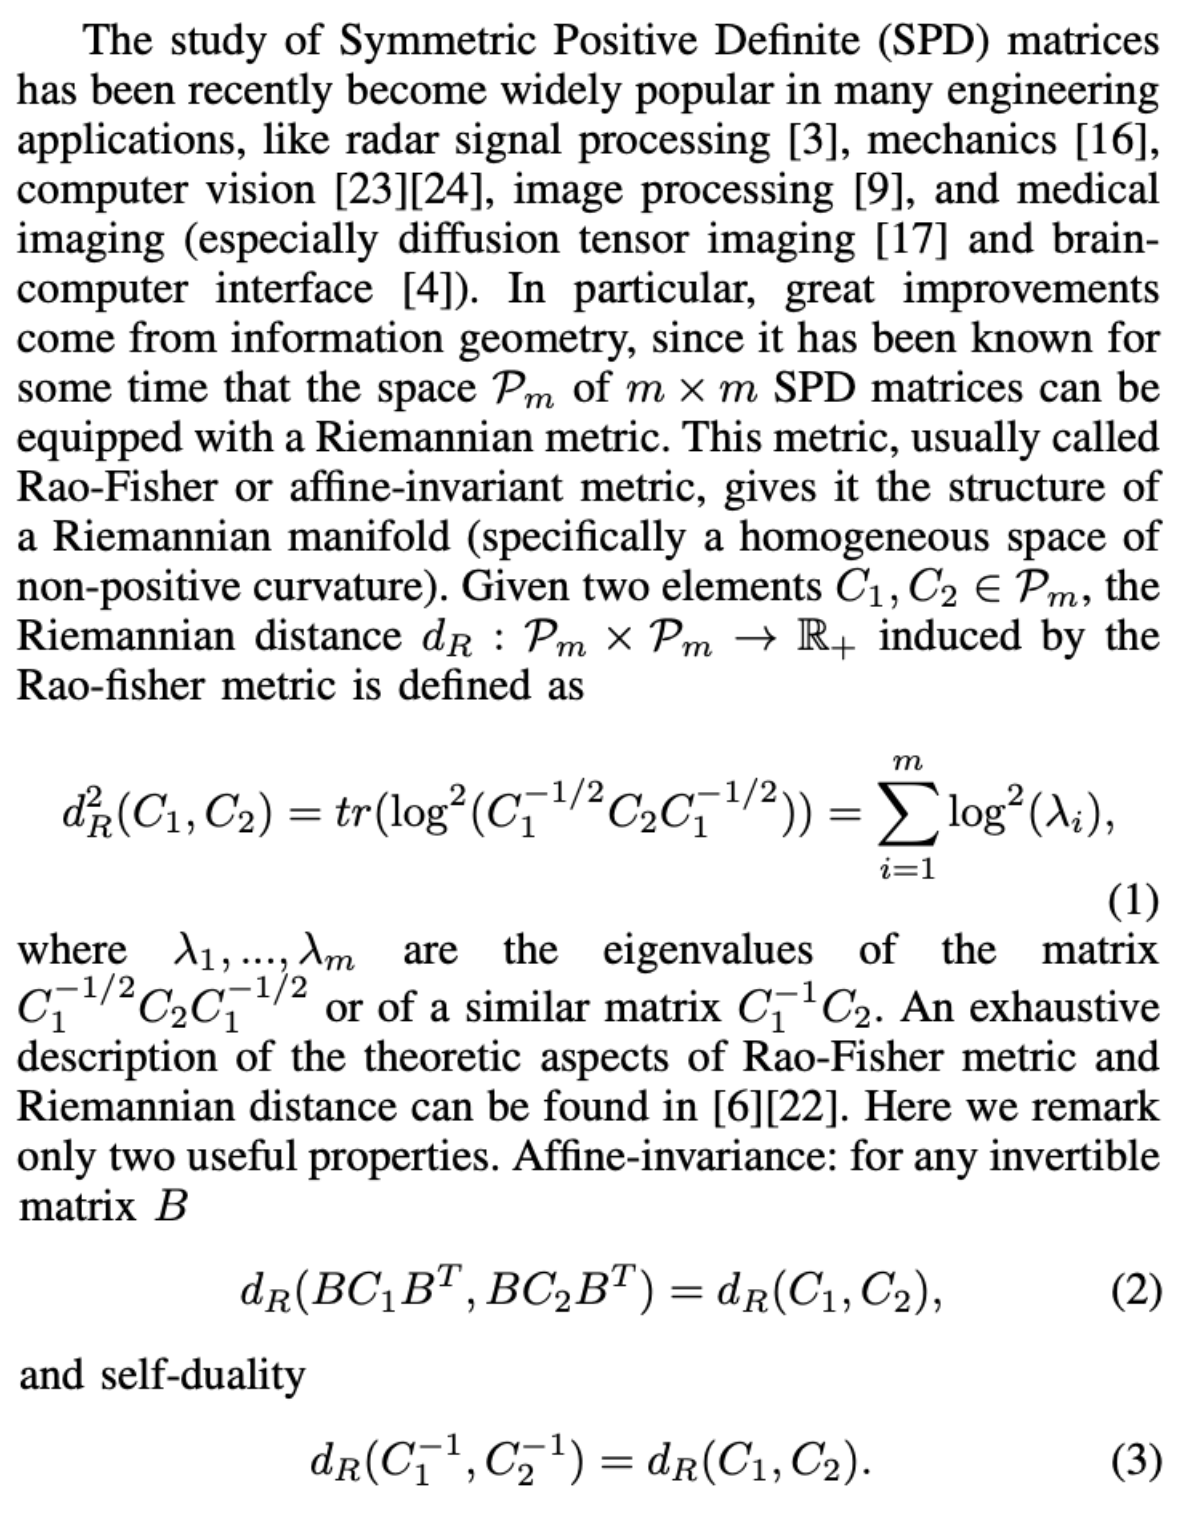
\includegraphics[width=0.8\linewidth]{figs/page-01-paragraph-01.png}}
  \vspace{1em}
\end{center}

A modelagem matemática do problema abordada pelos autores deriva os conceitos
da Geometria da Informação, área da matemática que utiliza ferramentas
geométricas no estudo de modelos estatísticos. Parte-se da variedade de
matrizes simétricas positivas-definidas $\mathcal{P}_m$ de dimensão $m \times
m$, sobre a qual define-se uma métrica Riemanniana. Introduzida em 1945 por
Rao, utilizando os fundamentos desenvolvidos por Ronald Fisher em 1921, esta
métrica tipicamente chamada de Rao-Fisher, define uma distância entre duas
distribuições de probabilidade, geodésicas, curvaturas e outras propriedades do
espaço~\cite{porto2013geometria}. Com esta métrica, definida pela Equação~(1),
a variedade adquire uma estrutura Riemanniana de um espaço homogêneo de
curvatura não-positiva.

Os autores destacam duas importantes propriedades da métrica de Rao-Fisher
$d_R^2 : \mathcal{P}_m \times \mathcal{P}_m \rightarrow \mathbb{R}_+$. A
primeira delas é a \textit{affine-invariance}, ou seja, a distância entre dois
elementos $C_1, C_2 \in \mathcal{P}_m$ não se altera o aplicar um conjunto de
transformações afins. A segunda propriedade é a \textit{self-duality}, onde a
distância entre $C_1^{-1}$ e $C_2^{-1}$ é a mesma que entre $C_1$ e $C_2$.  

\begin{center}
  \vspace{1em}
  \frame{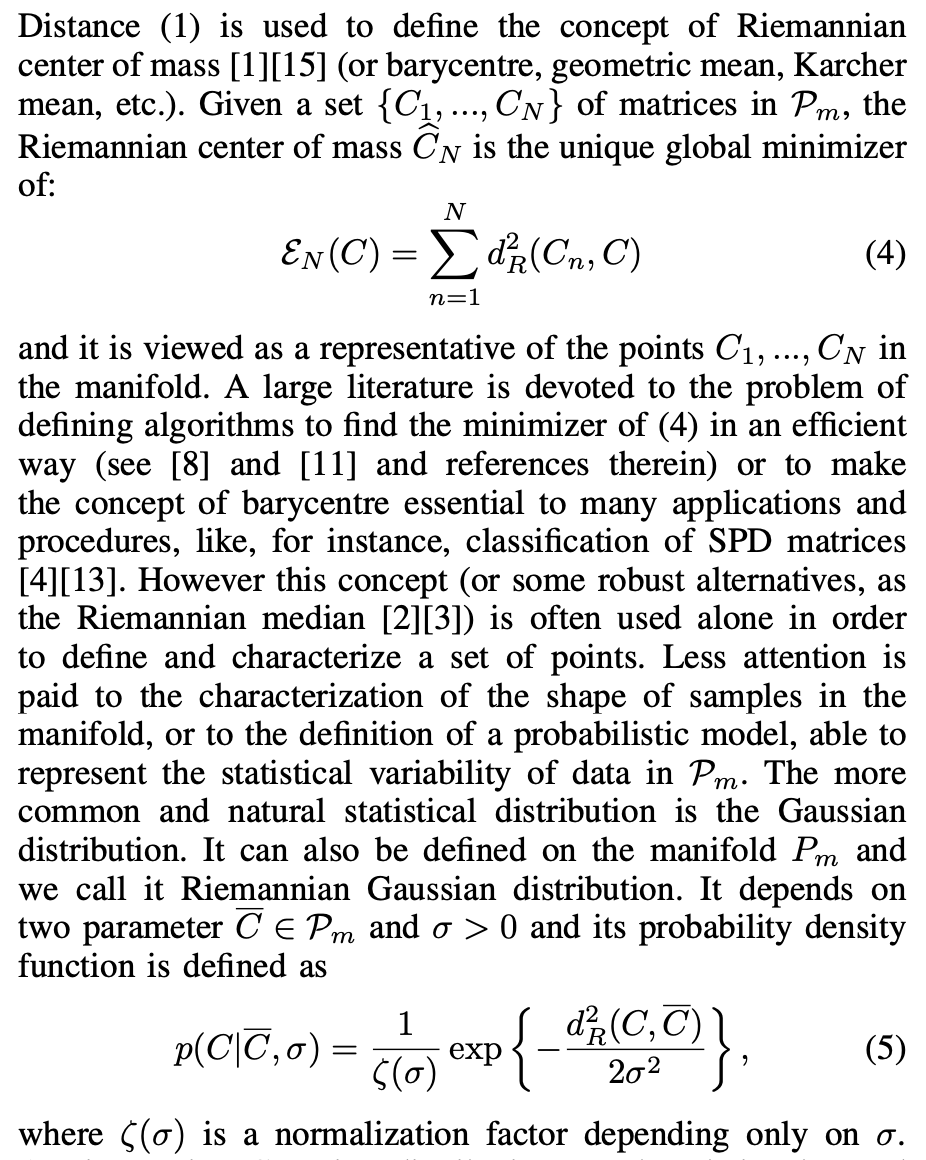
\includegraphics[width=0.8\linewidth]{figs/page-01-paragraph-02.png}}
  \vspace{1em}
\end{center}

A distância $d^2_R$ expressa pela Equação~(1), portanto, define o conceito de
centro de massa Riemanniano (ou baricentro, centro geométrico), o qual é utilizado
para a classificação de matizes SPD, dentre outras aplicações. Este centro de
massa, denotado por $\hat{C_N}$, é único e é dado pelo mínimo global da
Equação~(4). Várias técnicas tem sido empregadas para se encontrar este
minimizador. Como métodos de primeira ordem, pode-se citar o \textit{Steepest
Descent Method} e o \textit{Conjugate Gradient Method}. Também destacam-se
métodos de segunda ordem baseados na região de confiança (\textit{Trust region
method}) com suas variantes \textit{Exact Hessian}, \textit{Hessian by
decomposition}, \textit{Hessian by approximation} e ainda o
\textit{Broyden–Fletcher–Goldfarb–Shanno} (BFGS).

Entretanto, o conceito de centro de massa Riemannian tem sido amplamente
utilizado para definir e caracterizar um conjunto de pontos. Pouca atenção
tem-se dado para a caracterização da forma (ou \textit{shape}) das amostras na
própria variedade Riemanniana, o que possibilitaria caracterizar o modelo
probabilístico que governa os dados em $\mathcal{P}_m$.

Neste contexto de estatística, o modelo de distribuição de probabilidades
mais comum e naturalmente utilizado nas mais diversas áreas da ciência é o
modelo Gaussiano. Este modelo é dotado de particular notoriedade em virtude do
\textit{Teorema Central do Limite}, o qual estabelece que quando variáveis
aleatórias independentes são somadas, a distribuição de probabilidades
resultante tende a uma distribuição normal, ou
Gaussiana~\cite{fischer2010history}. Esta distribuição é parametrizada por
apenas duas quantidades, a média e a variância da variável aleatória.

Definido este modelo de distribuição de probabilidades na variedade
$\mathcal{P}_m$, tem-se então uma distribuição Gaussiana Riemanniana dada pela
Equação~(5), a qual depende da média $\bar{C} \in \mathcal{P}_m$ e da variância
$\sigma > 0$.

\begin{center}
  \vspace{1em}
  \frame{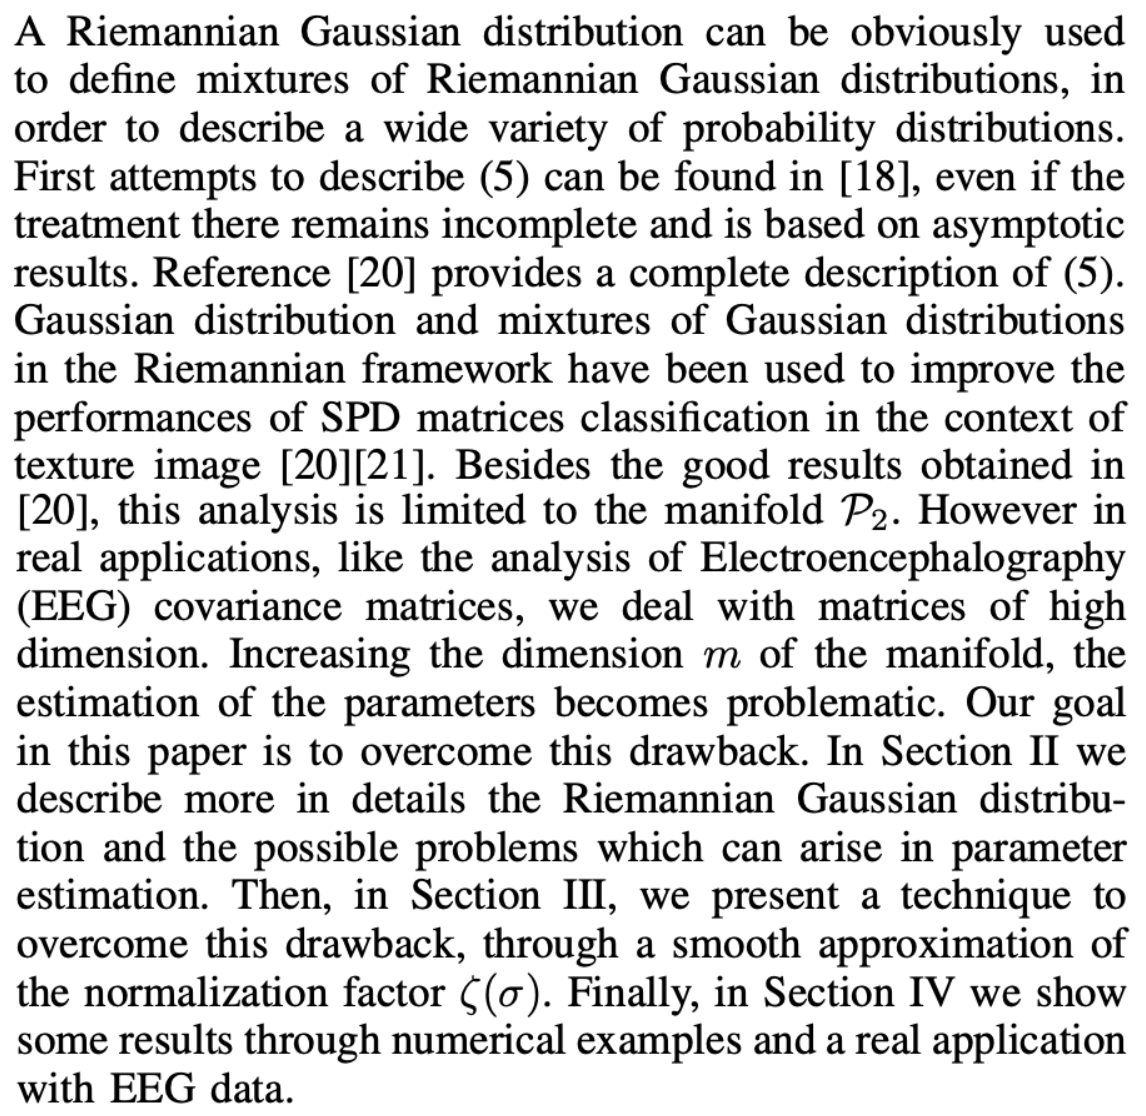
\includegraphics[width=0.8\linewidth]{figs/page-01-paragraph-03.png}}
  \vspace{1em}
\end{center}

O modelo de distribuição Gaussiana Riemanniana pode estendido para combinações
de distribuições Gaussianas Riemannianas, útil para descrever uma ampla
variedade de modelos probabilísticos. Estas construções tem sido utilizadas
para melhorar a performance de classificação de matrizes SPD no contexto de
imagens texturizadas, porém apesar dos bons resultados apresentados na
literatura, as análises até aqui tem se limitado em variedades de apenas duas
dimensões ($\mathcal{P}_2$). Contudo, para muitos outros problemas práticos,
como a análise de matrizes de covariância em Eletroencefalografia, lida-se com
fenômenos de alta dimensão onde o problema de estimação de parâmetros se torna
mais desafiador. Este trabalho se insere neste contexto, apresentando técnicas
para superar estas limitações.


\section{Commented and Expanded Section 2: Riemannian Gaussian Distribution}
Nesta seção os conceitos de Distribuição Gaussiana Riemanniana serão derivados
bem como os possíveis problemas que podem surgir na estimação de parâmetros.

\begin{center}
  \vspace{1em}
  \frame{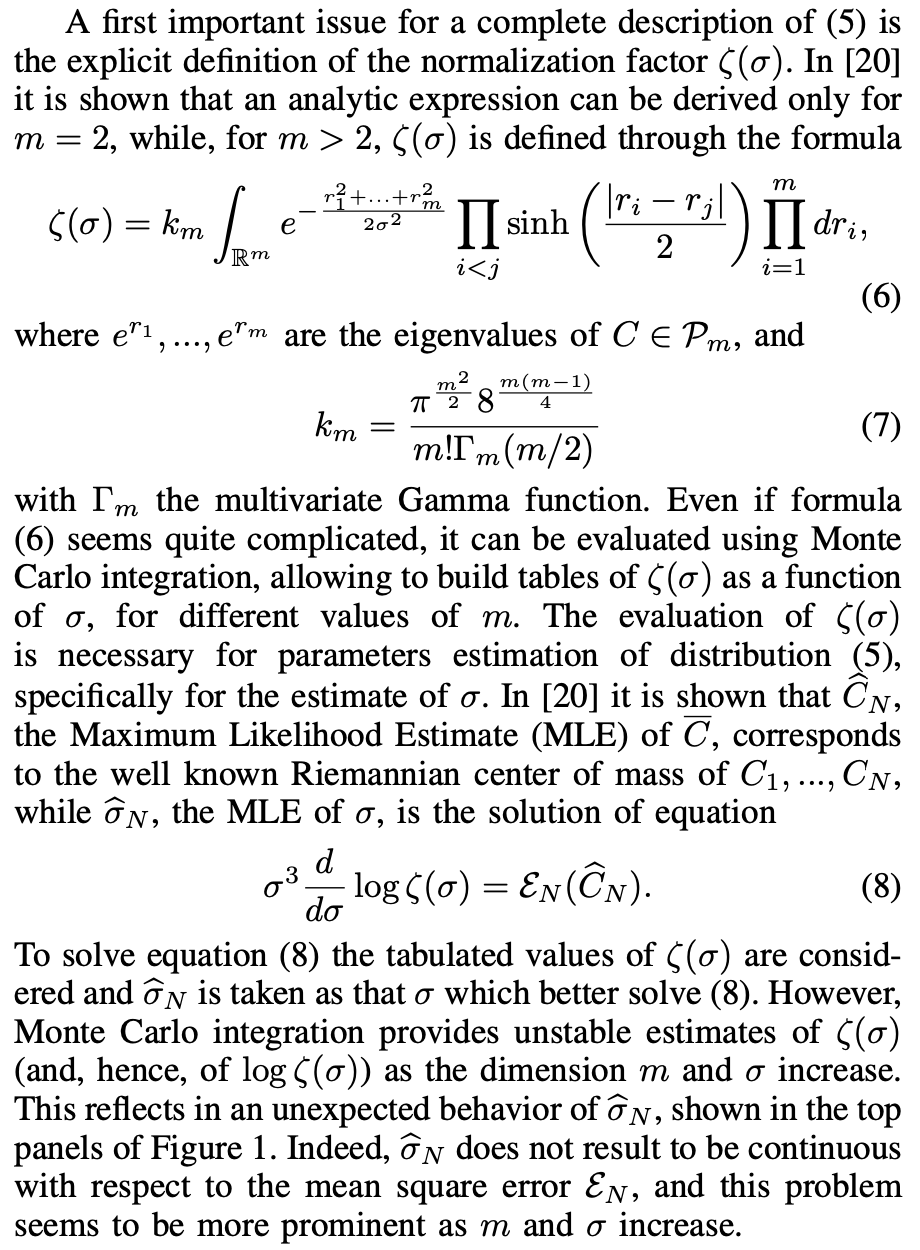
\includegraphics[width=0.8\linewidth]{figs/page-02-paragraph-01.png}}
  \vspace{1em}
\end{center}

No contexto de estimação de parâmetros de variáveis aleatórias Gaussianas,
busca-se estimar a média e a variância $\sigma$ da distribuição, uma vez que
este modelo pode ser totalmente caracterizado por estas duas
quantidades~\cite{kay}. Para este fim, diversos estimadores podem ser
encontrados na literatura, tanto de natureza linear (\textit{Best Linear
Unbiased Estimator}, \textit{Least Squares}, \textit{Wiener Filter}), quanto
não-linear (\textit{General Minimum Variance Estimator}, \textit{Bayesian
Estimators})\cite{kay,haykin}.

Entretanto, para problemas de alta dimensão, encontrar uma formulação fechada
para a distribuição Gaussiana em função do parâmetro desconhecido $\sigma$
torna-se um desafio. A busca por estimadores ótimos naturalmente é desenvolvida
na direção de se encontrar um minimizador para uma função de custo que,
tipicamente, depende do modelo da distribuição dos dados\cite{kay}. Esta busca
é em muito facilitada quando a função de custo é mais matematicamente tratável.
Contudo, dependendo da natureza do problema, nem sempre é possível obter uma
formulação analítica simplificada como entrada para o desenvolvimento de
estimadores, recorrendo-se à alternativas numéricas para contornar esta
limitação.

Os autores evidenciam este problema na Equação~(6), onde pode-se notar
a complexidade da formulação do fator de normalização $\zeta(\sigma)$. A
técnica utilizada para avaliar $\zeta(\sigma)$ foi através da tabulação do
valor da função para alguns valores de $\sigma$ utilizando integrações de Monte
Carlo.  Este método de integração numérica utiliza números aleatórios para
aproximar o valor da integral multivariada~(\cite{caflisch1998monte}).

A avaliação do valor de $\zeta(\sigma)$ é de fundamental importância para
estimar o parâmetro desconhecido $\sigma$ (variância da distribuição).
 Um estimador tipicamente empregado para estimação de parâmetros
de distribuições normais é o Estimador de Máxima Verossimilhança (MLE), o qual
estima os valores dos diferentes parâmetros do modelo estatístico de maneira a
maximizar a probabilidade dos dados observados, ou seja, busca-se parâmetros
que maximizem a função de verossimilhança. Geralmente, a função de
verossimilhança é dada pelo do logaritmo da função dos parâmetros
desconhecidos. A estimativa MLE da variância $\hat{\sigma_N}$ é dada pela
solução da Equação~(8). Note que esta equação depende do valor de
$\zeta(\sigma)$, o qual foi tabelado pela integração de Monte Carlo.
Entretanto, esta aproximação apresenta instabilidades que degradam a eficiência
da estimação $\hat{\sigma_N}$. O problema fica ainda pior quando se aumenta o
valor da variância $\sigma$ ou da dimensão da variedade $m$.  

\begin{center}
  \vspace{1em}
  \frame{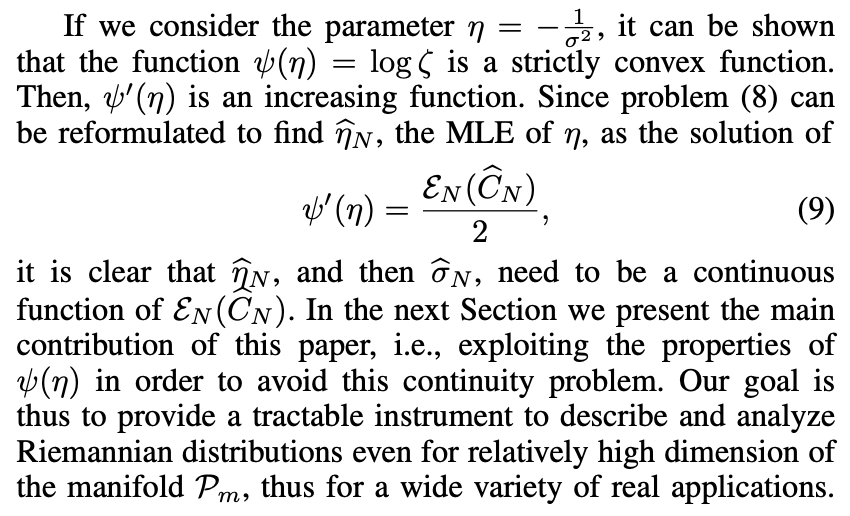
\includegraphics[width=0.8\linewidth]{figs/page-02-paragraph-02.png}}
  \vspace{1em}
\end{center}

Aplicando-se uma transformação não-linear no parâmetro desconhecido $\sigma$,
pode-se obter um função estritamente convexa sobre o parâmetro de forma com que
sua derivada é uma função crescente (Equação~(9)). Esta manipulação matemática
apresenta algumas vantagens do ponto de vista de otimização que tornam o
problema mais tratável. Em especial, esta reformulação irá prover um
instrumental matemático que possibilitará a análise de distribuições
Riemannianas em variedades de altas dimensões, com ampla aplicação em problemas
reais.

\section{Commented and Expanded Section 3: Parameters Estimate}
Nesta seção é apresentada uma técnica de estimação de parâmetros de
distribuições Gaussianas multivariadas aplicadas em variedades Riemannianas.

\begin{center}
  \vspace{1em}
  \frame{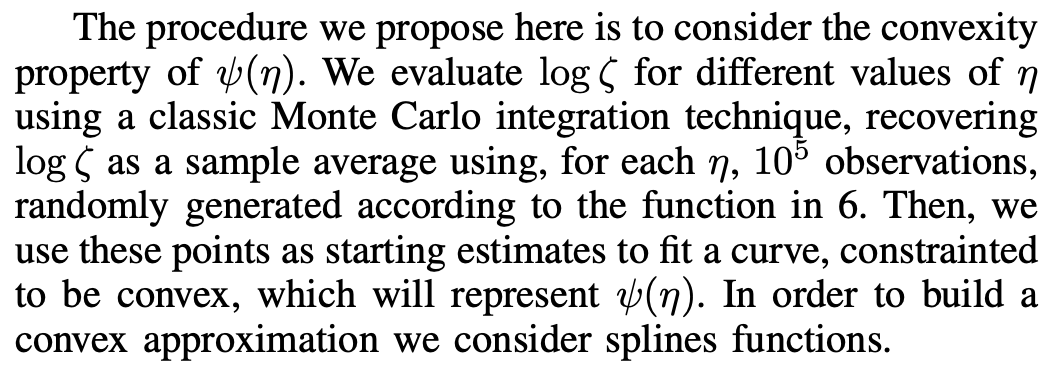
\includegraphics[width=0.8\linewidth]{figs/page-02-paragraph-03.png}}
  \vspace{1em}
\end{center}

Vale reforçar que o grande desafio de se estimar parâmetros de distribuições
Gaussianas Riemannianas de alta dimensão é devido à complexidade do modelo
analítico que descreve matematicamente esta distribuição. Tipicamente, quando
a solução analítica é impraticável ou demasiadamente complexa, recorre-se à
técnicas numéricas que possibilitam encontrar aproximações para a solução do
problema em questão.

Para estimar a variância $\sigma$ da distribuição Gaussian Riemanniana de alta
dimensão, os autores propõem uma técnica numérica que proverá uma aproximação
para esta quantidade. Parte-se inicialmente de uma transformação não-linear
$\eta = \frac{-1}{\sigma^2}$ que possibilita a construção de uma função de
verossimilhança $\psi(\eta) = \log \zeta(\eta)$ estritamente convexa, ou seja,
$\psi^{''}(\eta) > 0\,, \forall \eta$. Posteriormente, a função
$\log \zeta(\eta)$ é avaliada numericamente para alguns valores de $\eta$,
utilizando integrações de Monte Carlo. Em posse destas aproximações, a função
$\phi(\eta)$ pode ser finalmente interpolada através de \textit{splines cúbicos}. 

\begin{center}
  \vspace{1em}
  \frame{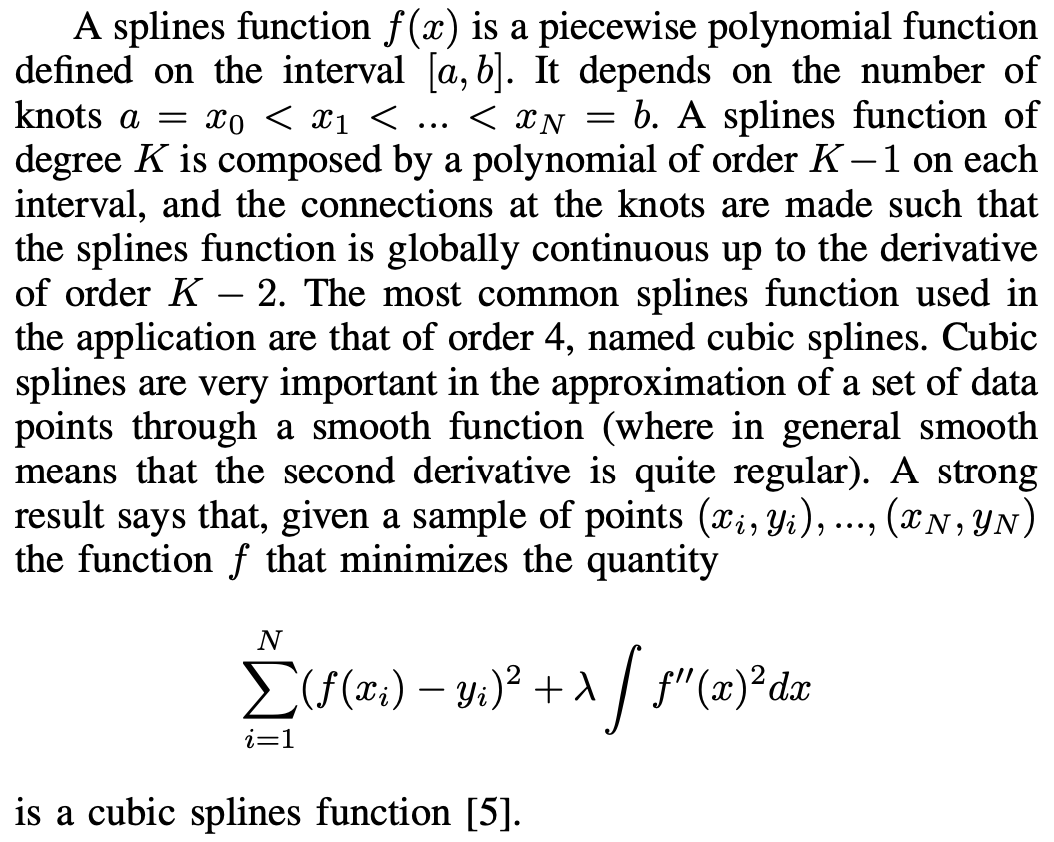
\includegraphics[width=0.8\linewidth]{figs/page-02-paragraph-04.png}}
  \vspace{1em}
\end{center}

Em matemática, os \textit{Splines} são um tipo especial de função defina por
dois ou mais pontos de controle, cujo grau é escolhido por projeto. Através
desta técnica, é possível construir uma curva que passa por todos os pontos
de controle, ou seja, uma curva que interpola os intervalos entre estes pontos
~\cite{ruggiero1996calculo}. Nas splines cúbicas, determina-se um
polinômio interpolador ou aproximador de terceiro grau com restrições que
garantam uma curva suave, ou seja, onde a primeira e segunda derivadas são
contínuas.

\begin{center}
  \vspace{1em}
  \frame{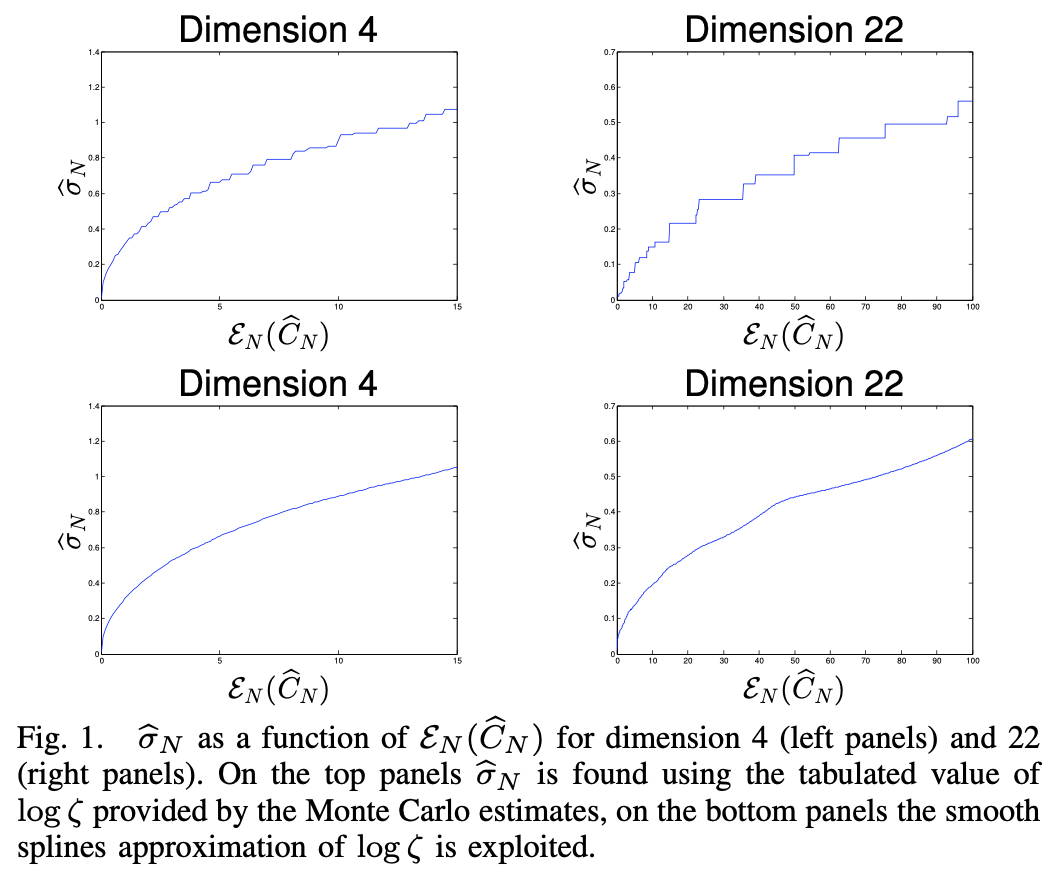
\includegraphics[width=0.8\linewidth]{figs/figure-01.png}}
  \vspace{1em}
\end{center}

A figura acima mostra o valor estimado da variância da distribuição Gaussiana
Riemanniana $\hat{\sigma}_n$ em função do erro médio quadrático (SMR)
$\mathcal{E}_N(\hat{C}_N)$ para quatro condições diferentes. Os gráficos a
esquerda referem-se à uma variedade $\mathcal{P}_m$ de dimensão $m=4$ e os
gráficos a direita de dimensão $m=22$. Os gráficos superiores utilizam os
valores tabulados através do estimador de Monte Carlo. Os gráficos inferiores,
os valores foram aproximados através dos splines cúbicos.

Para ambos os estimadores, pode-se notar diretamente que o erro médio
quadrático cresce em função da variância. Entretanto, a função variância
aproximada pelo estimador de Monte Carlo é descontínua dentro do intervalo de
operação, apresentando variações abruptas ao longo da curva. Para alta
dimensão, este problema é ainda mais evidente e intensificado. Em contra
partida, a aproximação por splines cúbicos resulta em uma função aproximada
mais suave em toda a faixa de operação, tanto em baixa quanto em alta dimensão.
Este resultado se deve às restrições se suavidade impostas na técnica dos
splines cúbicos, que garantem a existência e a continuidade da primeira e
segunda derivadas.  

\begin{center}
  \vspace{1em}
  \frame{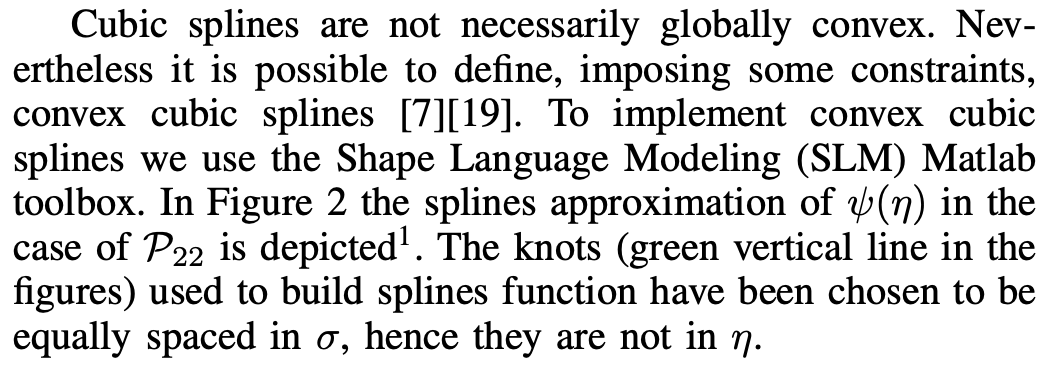
\includegraphics[width=0.8\linewidth]{figs/page-02-paragraph-05.png}}
  \vspace{1em}
\end{center}

Por definição, os splines cúbicos não são globalmente convexos, ou seja,
de forma geral, não existem restrições quanto ao módulo da segunda derivada
em todo o domínio da interpolação. Portanto, pode-se construir os splines
cúbicos através de convoluções de forma a preservar a convexidade global
do polinômio aproximador (\textit{fit})~\cite{convexsplines}. Os autores
implementaram esta técnica de splines por convoluções com o auxílio da
ferramenta SML do Matlab\cite{d2009slm}, a qual proporciona a construção de
curvas a partir de pontos de forma mais simplificada.

\begin{center}
  \vspace{1em}
  \frame{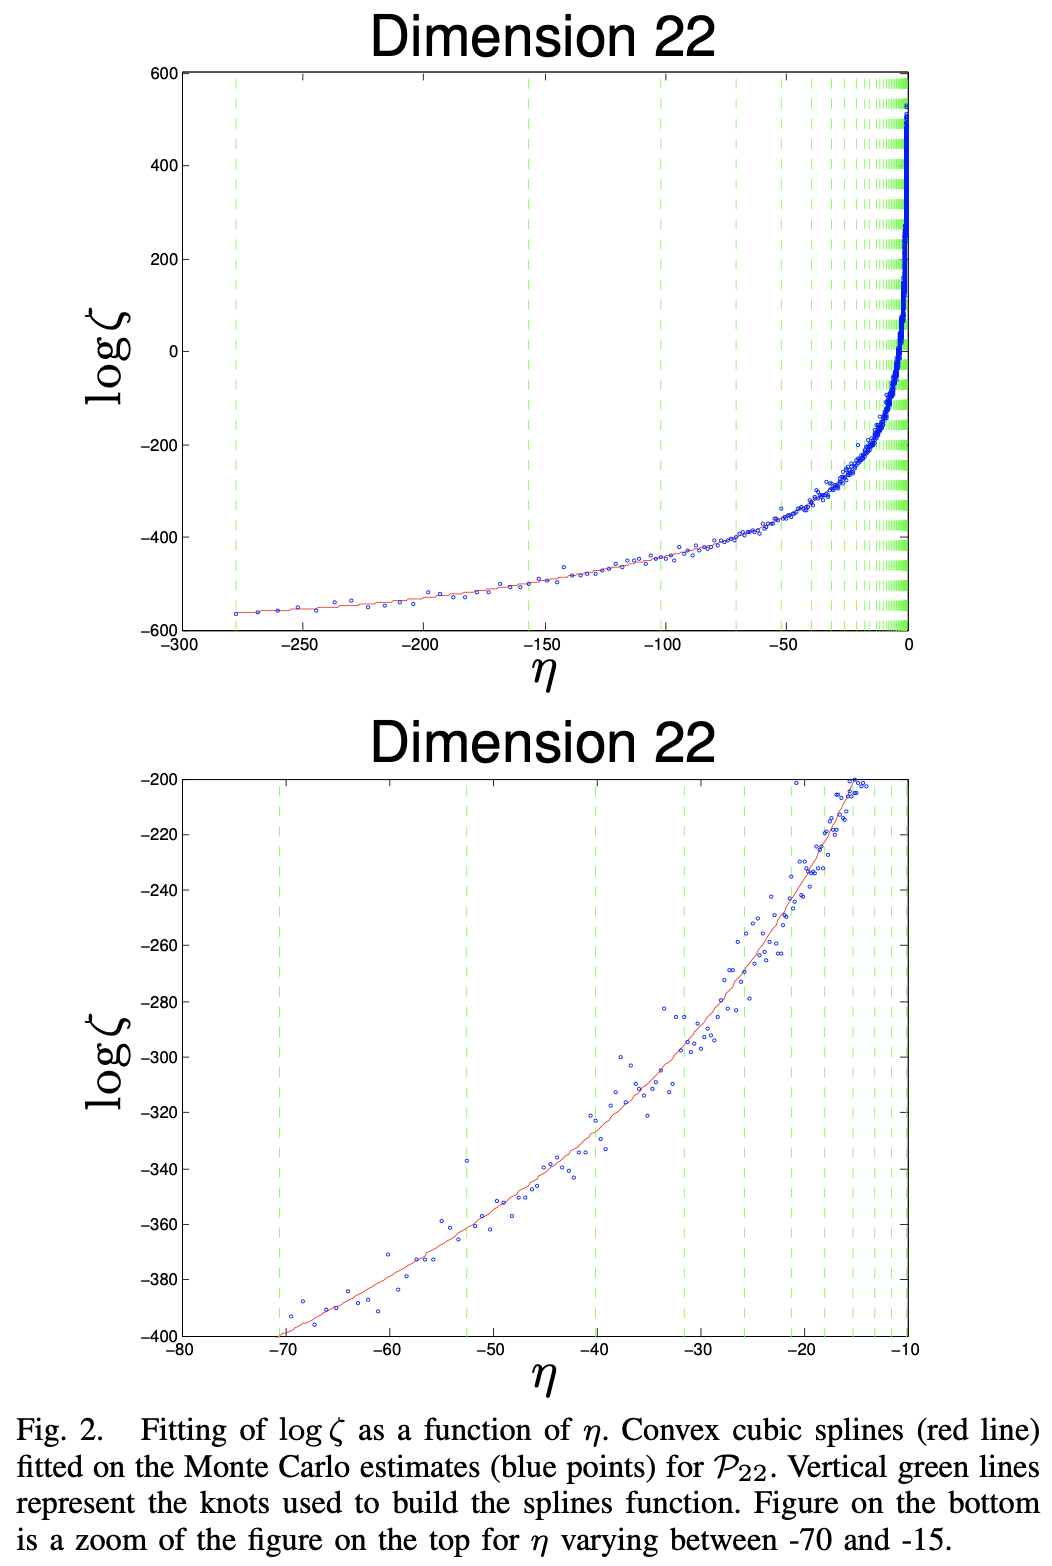
\includegraphics[width=0.8\linewidth]{figs/figure-02.png}}
  \vspace{1em}
\end{center}

A figura acima mostra em azul o conjunto de pontos da função
$\psi(\eta) = \log \zeta(\eta)$ aproximados pelo método de Monte Carlo.
A função que aproxima a distribuição dos pontos (função de \textit{fitting})
está representada em vermelho. Vale notar que, para este caso, a dimensão da
variedade $P_m$ é $m=22$. Esta função de fitting foi construída através dos
splines cúbicos a partir de nós de controle igualmente espaçados (linhas
verticais em verde), utilizando a restrição de convexidade global citada
anteriormente. Nota-se visualmente que a função de fitting consegue modelar
bem conjunto de dados, porém os autores não apresentam nenhuma medida de
concordância ou alguma análise de erro de aproximação. Este tipo de análise
qualitativa é fundamental para se verificar o quão bem um modelo representa
os dados estudados.

\begin{center}
  \vspace{1em}
  \frame{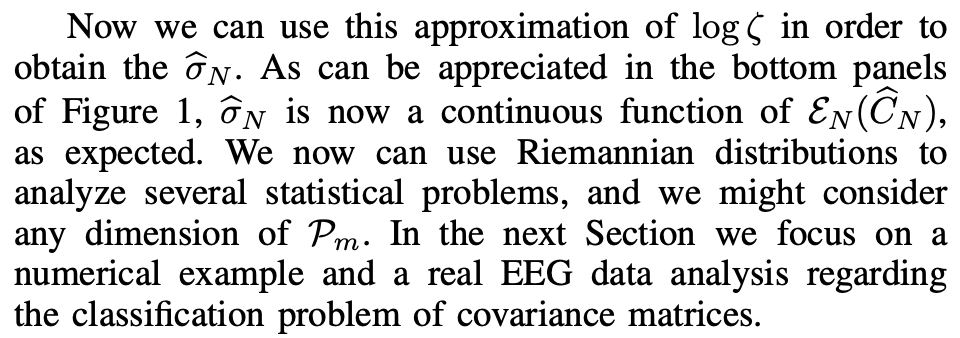
\includegraphics[width=0.8\linewidth]{figs/page-03-paragraph-01.png}}
  \vspace{1em}
\end{center}

Relembrando, o objetivo é estimar a variância $\hat{\sigma}_N$ da distribuição
Gaussiana Riemannian $\zeta(\sigma)$ (Equação~(6)) através da maximização da
função de verossimilhança $\psi(\eta)$ (Equação~(9)), a qual depende do
conhecimento de $\log \zeta(\eta)$, cuja solução analítica é impraticável.
Para contornar o problema, a função $\log \zeta(\eta)$ foi aproximada para
alguns valores de $\eta$ através do método de Monte Carlo e, em posse destes
pontos aproximados, uma função de fitting contínua foi construída pelo métodos
dos splines cúbicos globalmente convexos. Desta forma, tem-se todos os
elementos para estimar a variância $\hat{\sigma}_N$.

\section{Commented and Expanded Section 4: Results}
Nesta seção os resultados obtidos nas análises de sinais com EEG utilizando
técnicas baseadas em Variedades Riemannianas são apresentados.

\begin{center}
  \vspace{1em}
  \frame{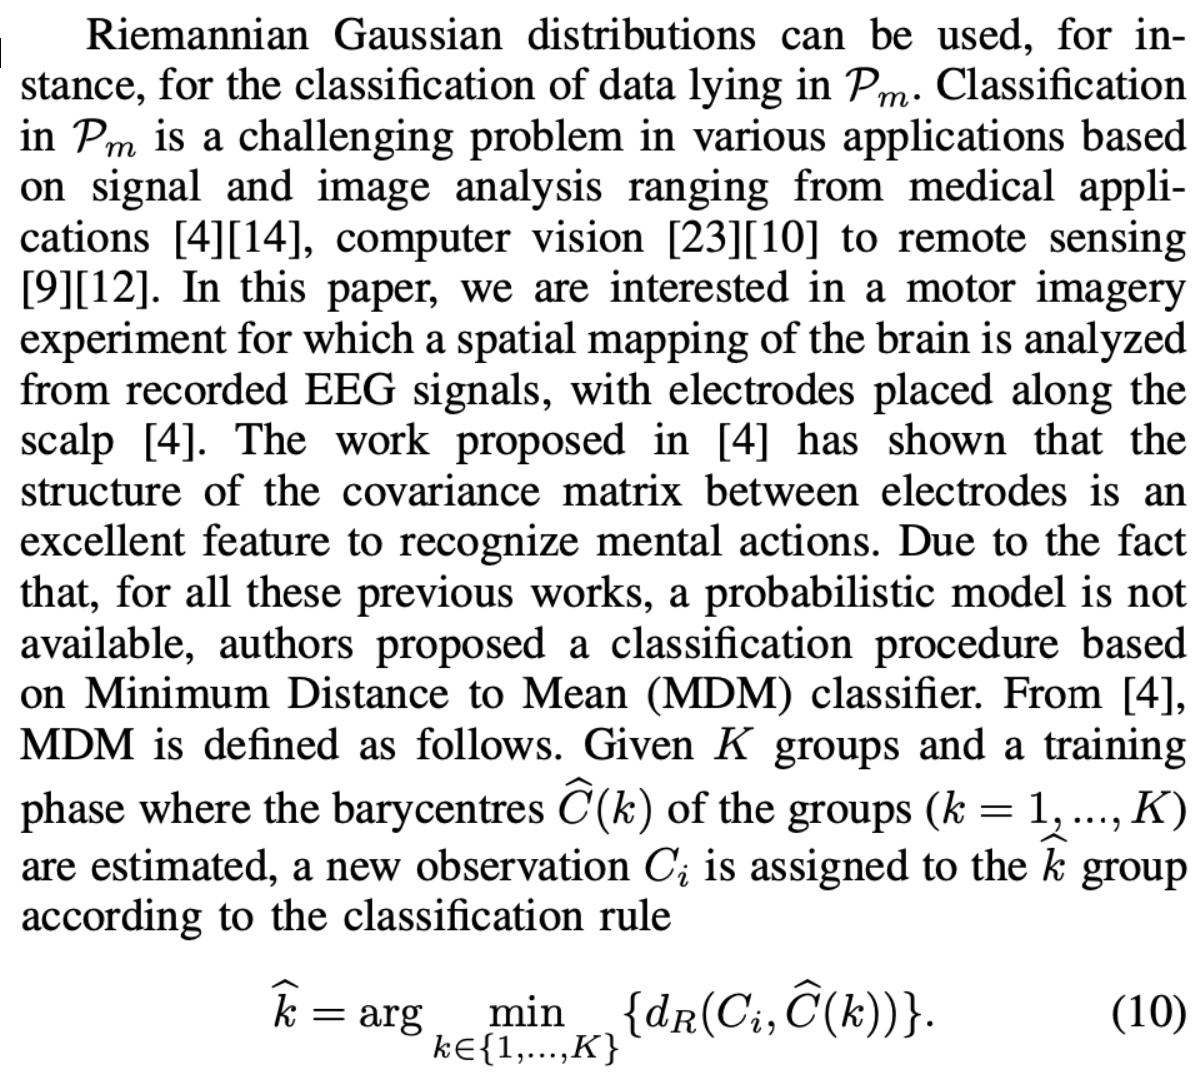
\includegraphics[width=0.8\linewidth]{figs/page-03-paragraph-02.png}}
  \vspace{1em}
\end{center}

Como ambiente experimental, os autores utilizam sinais de Eletroencefalografia
(EEG) capturados através de eletrodos localizados ao longo do couro cabeludo de
um indivíduo. Através destes sinais, busca-se analisar o mapeamento espacial
através da matriz de covariância entre os eletrodos, a qual pode ser utilizada
para caracterizar padrões mentais. Portanto, trata-se de um problema de
classificação onde o modelo de distribuição Gaussiana Riemanniana pode ser
útil.

A geometria Riemanniana é um ramo da geometria diferencial que estuda
variedades suaves, espaços curvos com geometrias peculiares. Nestes espaços as
noções de ângulos, caminho mais curto entre dois pontos, distâncias, centro de
massa de vários pontos, etc., permitem estudar propriedades analíticas de
operadores matemáticos de uma perspectiva geométrica, tornando-os acessíveis à
intuição~\cite{levi1925lezioni,congedo2019riemannian}.

No contexto de Eletroencefalografia multivariada, a variedade de matrizes
simétricas positivas-definidas $\mathcal{P}_m$ tem se mostrado muito útil, uma
vez que dados de EEG em janelas de tempo finitas podem ser efetivamente
mapeados como pontos nesta variedade através da estimação de parâmetros de sua
matriz de covariância. Esta abordagem levou à introdução de classificadores com
características notáveis em comparação com o estado da
arte~\cite{congedo2019riemannian}.

Devido à complexidade de se determinar um modelo probabilístico que governa
o processo estocástico associado aos sinais de EEG, tipicamente adota-se um
procedimento de classificação baseada na Mínima Distância para a Média (da
sigla em inglês, MDM). Em particular, este classificado, embora não seja o mais
preciso entre os classificadores Riemannianos, destaca-se por sua simplicidade
e eficiência computacional. É um classificador totalmente determinístico e
livre de parâmetros, portanto, nenhum parâmetro precisa ser ajustado por
validação cruzada ou outros métodos que possam comprometer sua
generalização~\cite{congedo2019riemannian}.

O MDM é definido pela Equação~(10), onde dados os grupos $K$ e uma fase de
treinamento onde os baricentros $\hat{C}(k)$ dos grupos $(k=1,\ldots,K)$ são
estimados, associa-se uma nova observação $C_i$ ao grupo $\hat{K}$ de acordo
com a regra de classificação baseada na mínima distância $d_R$.

\begin{center}
  \vspace{1em}
  \frame{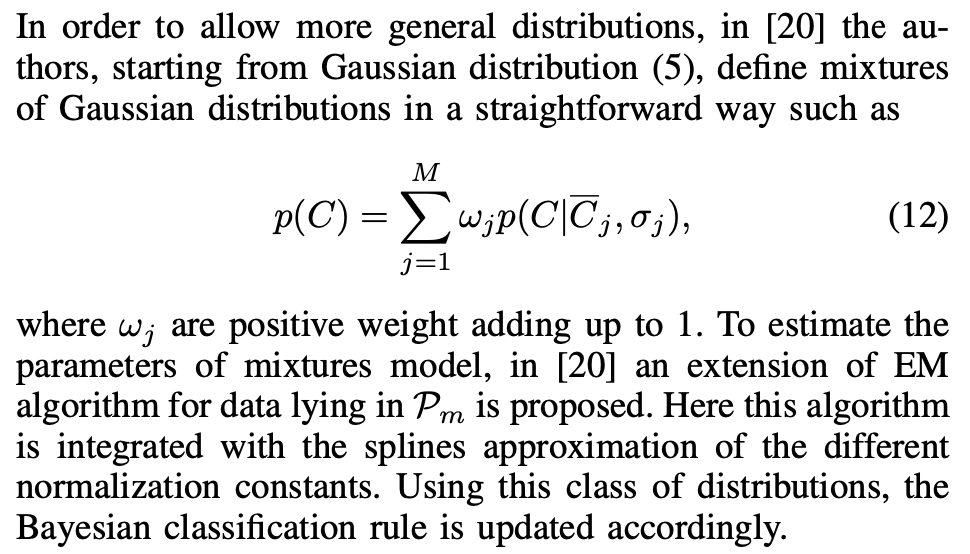
\includegraphics[width=0.8\linewidth]{figs/page-03-paragraph-03.png}}
  \vspace{1em}
\end{center}

Com o objetivo de possibilitar modelos de distribuição de probabilidade mais
gerais, os autores utilizam uma combinação linear de várias distribuições
Gaussianas (\textit{Gaussian Mixtures (GM)}), definida pela Equação~(12).
Uma extensão do algoritmo \textit{Expectation-Maximisation} (EM) é utilizada
para calcular as estimações de máxima verossimilhança dos parâmetros da
distribuição Gaussiana mista. Este algoritmo utiliza uma regra de classificação
ótima de Bayes, usando probabilidades de classificação a posteriori para melhorar
a eficiência de estimação.

\begin{center}
  \vspace{1em}
  \frame{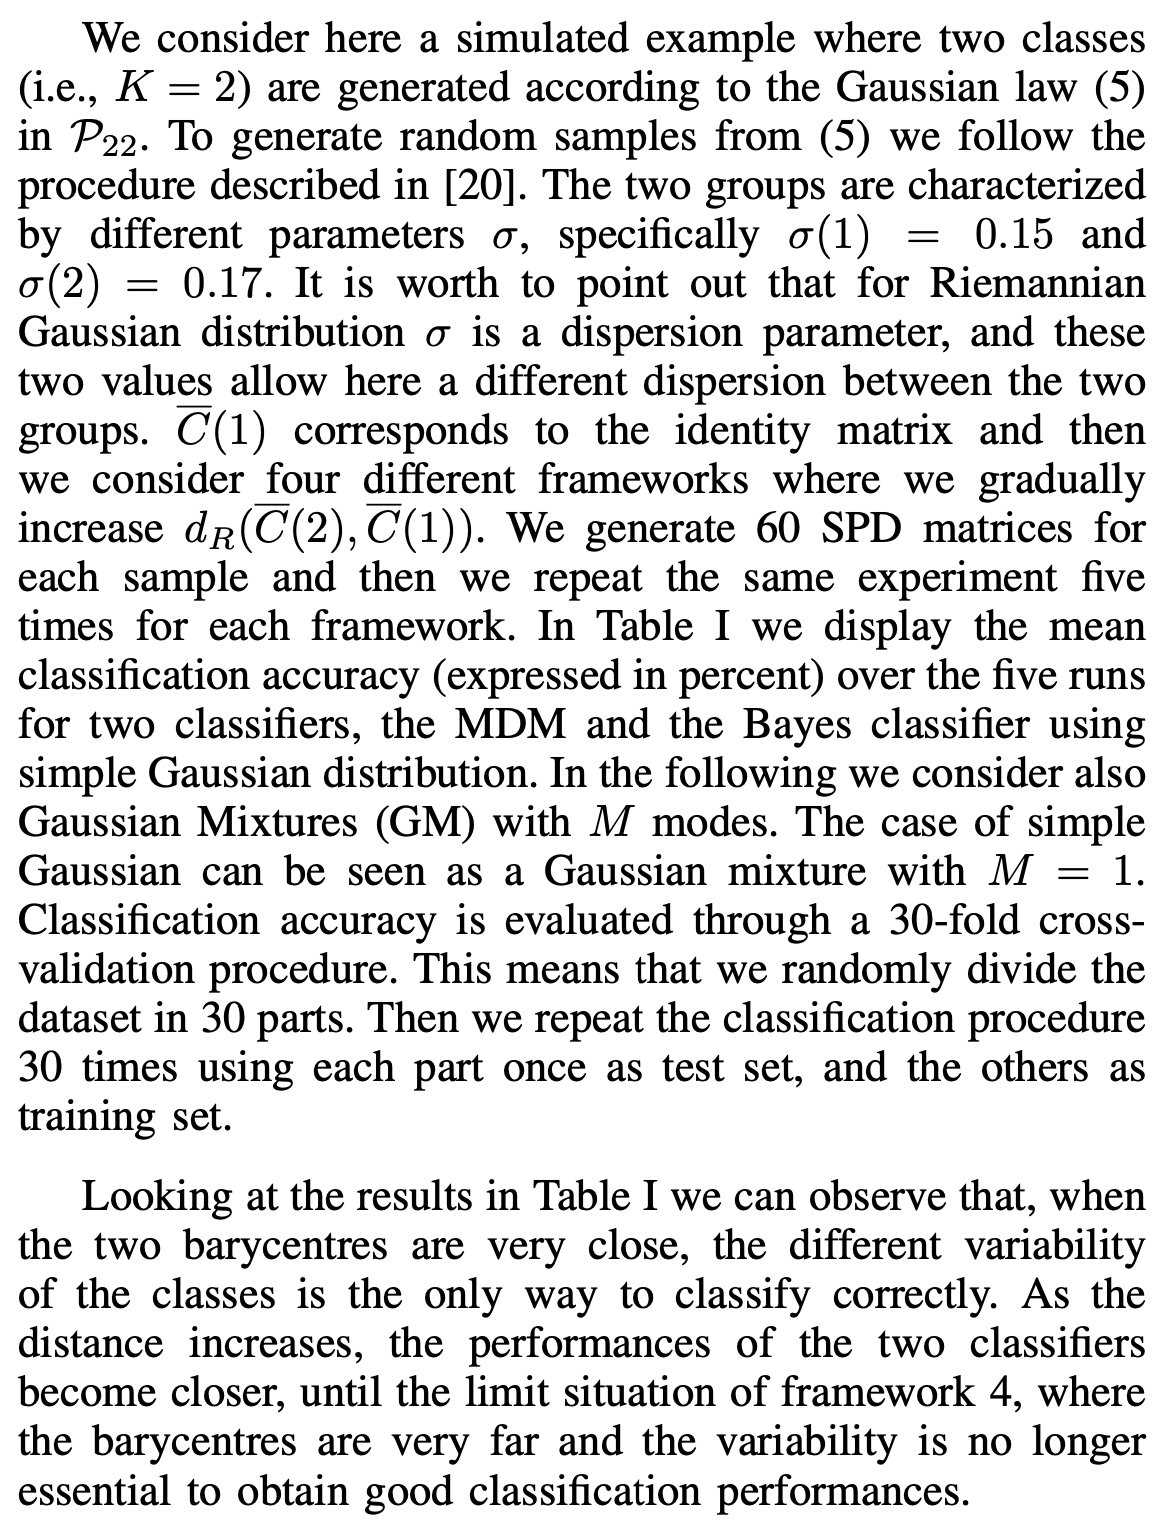
\includegraphics[width=0.8\linewidth]{figs/page-03-paragraph-04.png}}
  \vspace{1em}
\end{center}

Os autores utilizaram dois grupos ($K=2$), os quais são caracterizados por
valores de $\sigma$ distintos, sendo $\sigma(1) = 0.15$ e $\sigma(2) = 0.17$.
De forma análoga à distribuições Gaussianas em geral, o parâmetro $\sigma$
refere-se a dispersão, ou variância, dos dados na variedade Riemanniana.  
$\bar{C}(1)$ corresponde à matriz identidade e quatro diferentes cenários serão
considerados, incrementando gradualmente a distância
$d_R(\bar{C}(2), \bar{C}(1))$. Os autores geram 60 matrizes SPD para cada
amostra e repetem o mesmo experimento por cinco vezes para cada cenário.

\begin{center}
  \vspace{1em}
  \frame{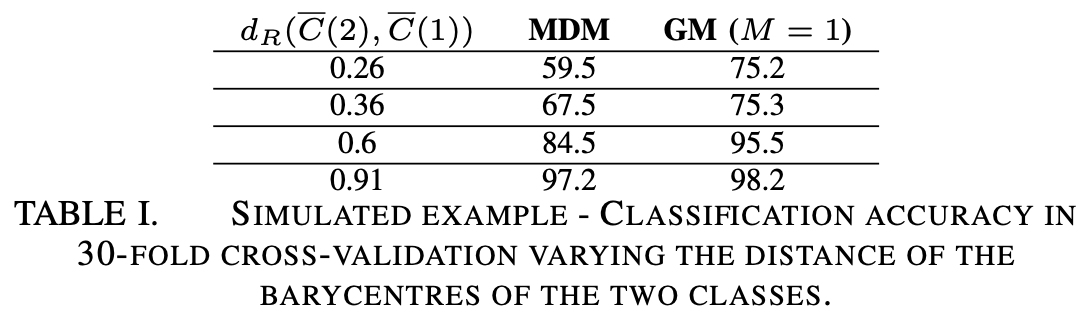
\includegraphics[width=0.8\linewidth]{figs/table-01.png}}
  \vspace{1em}
\end{center}

A tabela acima mostra a acurácia de classificação média em porcentagem das
cinco rodadas de cada um dos quatro cenários. São apresentados os resultados
de dois classificadores, o MDM e o classificador de Bayes utilizando uma
distribuição Gaussiana simples, ou seja, GM com $M=1$. Os resultados foram
obtidos através de um processo de validação cruzada, subdividindo o conjunto de
dados em 30 partes e repetindo o processo de classificação 30 vezes usando cada
parte como conjunto de teste e as demais como conjunto de treinamento.
Pode-se notar que o classificador de Bayes apresenta melhor eficiência em
termos de acurácia média para toda a faixa de distância avaliada, em especial
para os valores de baixa amplitude. Também vale notar que quando os dois
baricentros estão muito perto, ou seja, quando o valor de $d_R$ é pequeno,
as variantes de cada grupo são a única forma de classificar corretamente.
Conforme a distância $d_R$ aumenta, o desempenho dos dois classificadores se
aproxima, até a situação limite do cenário 4, onde os baricentros estão muito
distantes e a variabilidade não é mais essencial para obter bons desempenhos de
classificação.

\begin{center}
  \vspace{1em}
  \frame{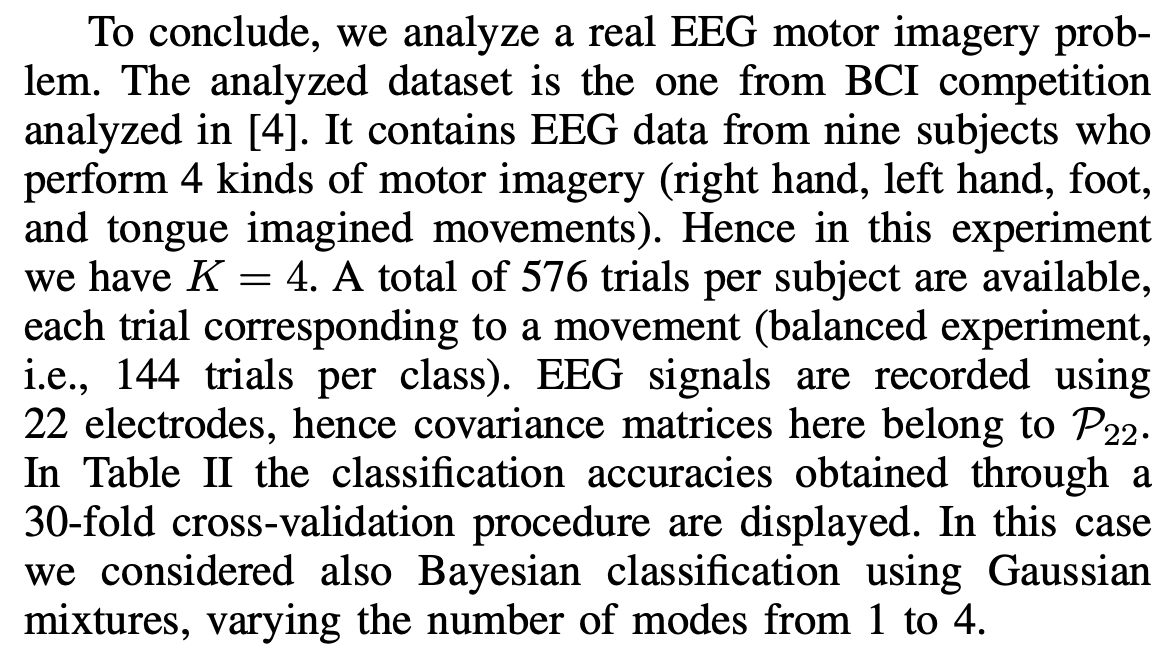
\includegraphics[width=0.8\linewidth]{figs/page-04-paragraph-01.png}}
  \vspace{1em}
\end{center}

Agora serão analisados dados reais de EEG de nove indivíduos que executam
quatro tipos de imagens motoras (movimentos imaginados da mão direita, mão
esquerda, pé e língua). Desta forma, neste experimento há quatro grupos de
classificação, ou seja, $K=4$. O conjunto de dados contém 144 amostras de cada
classe para cada um dos indivíduos. Estes sinais de EEG são capturados através
de 22 eletrodos, e portanto, as matrizes de covariância pertencem à variedade
$\mathcal{P}_{22}$.

\begin{center}
  \vspace{1em}
  \frame{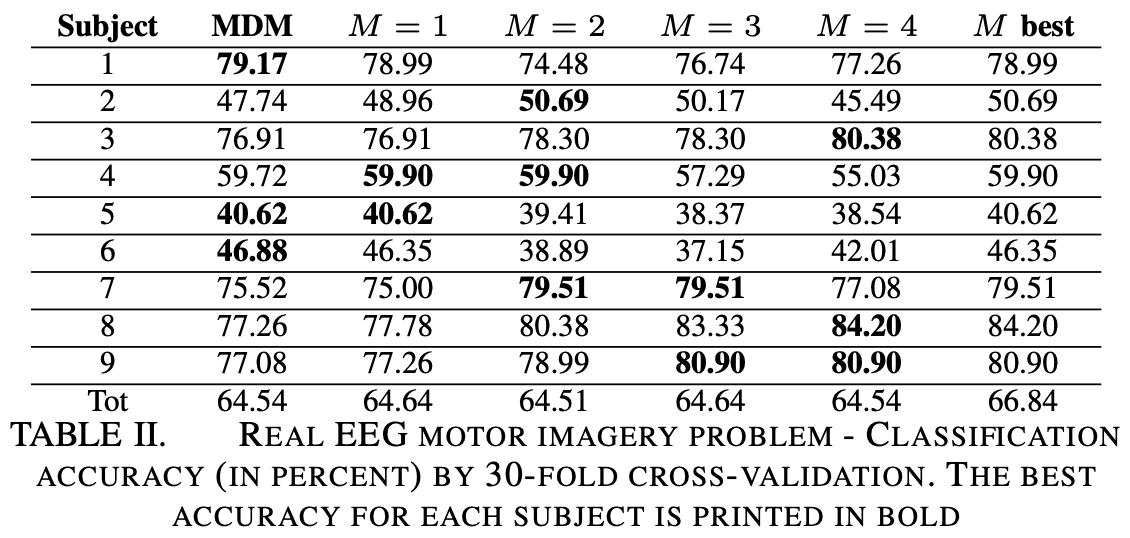
\includegraphics[width=0.8\linewidth]{figs/table-02.png}}
  \vspace{1em}
\end{center}

A tabela acima mostra a acurácia obtida através de um processo de validação
cruzada com 30 subdivisões, considerando o classificador MDM e o classificador
de Bayes utilizando uma distribuição Gaussiana Mista (GM) com $M$ variando de 1
a 4.

\begin{center}
  \vspace{1em}
  \frame{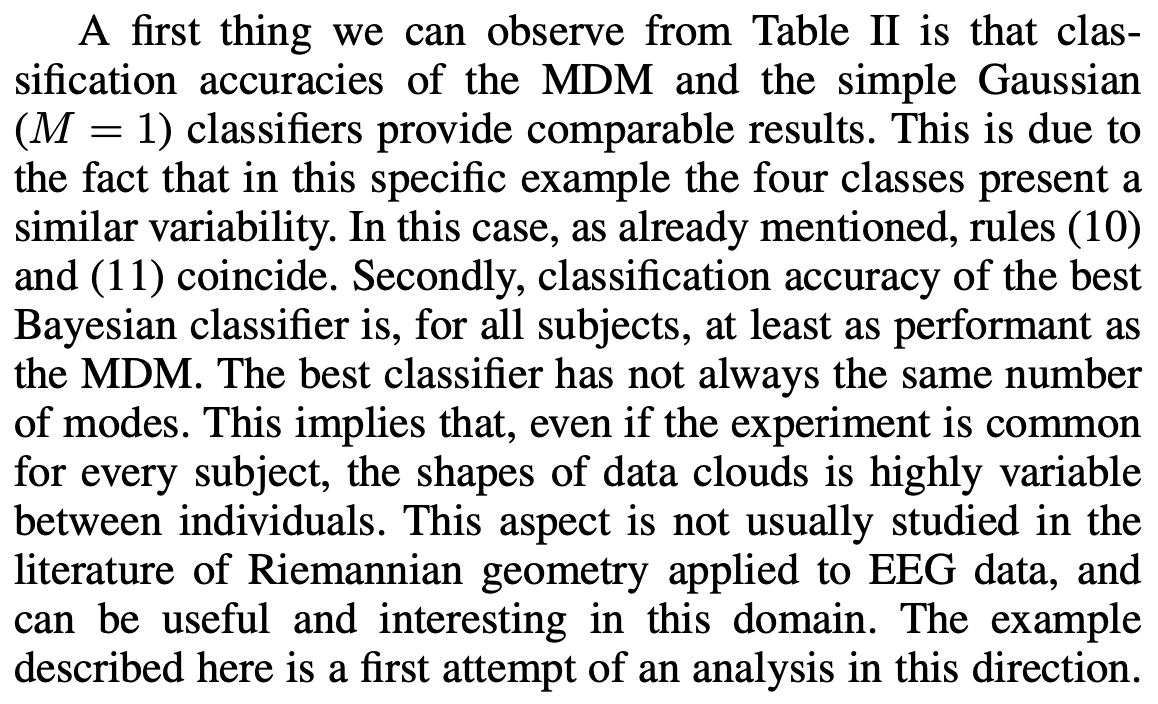
\includegraphics[width=0.8\linewidth]{figs/page-04-paragraph-02.png}}
  \vspace{1em}
\end{center}

Os resultados apresentados na Tabela 2 são interessantes em dois aspectos.
Primeiramente, os dados mostram que para todos os indivíduos, o classificador de
Bayes se mostrou pelo menos tão performático quanto o MDM\@. Segundo, os
resultados também mostram que o melhor classificador não está sempre associado
ao mesmo valor de $M$. Isto significa que, mesmo que o procedimento experimental
seja o mesmo para cada indivíduo, a variabilidade é alta, ou seja, a forma da
nuvem de dados na variedade Riemanniana é bem distinta entre os indivíduos.
Este aspecto ainda não foi amplamente estudado na literatura de Geometria
Riemanniana no contexto de EEG e pode ser um campo promissor para novos
estudos. Vale ressaltar que os resultados mostrados neste trabalho foram os
primeiros nesta direção.

\begin{center}
  \vspace{1em}
  \frame{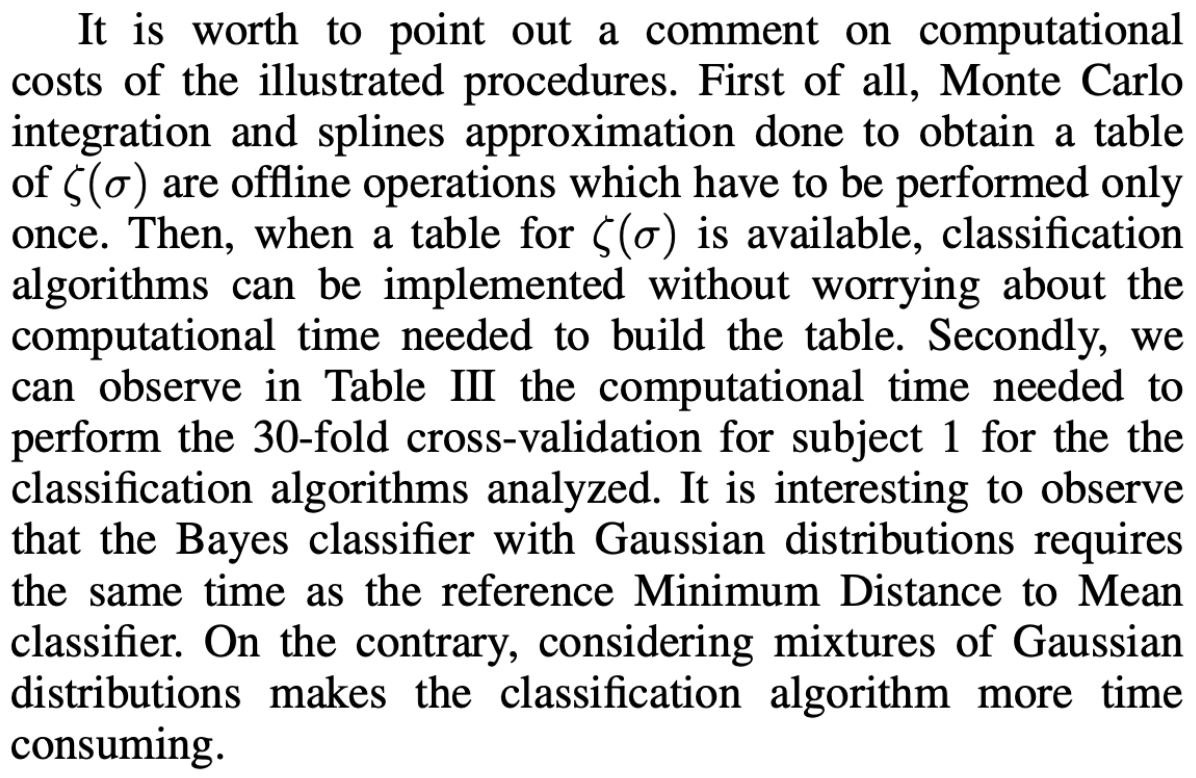
\includegraphics[width=0.8\linewidth]{figs/page-04-paragraph-03.png}}
  \vspace{1em}
\end{center}

Outro ponto que merece destaque é relacionado ao custo computacional dos
procedimentos aqui apresentados. A análise do tempo de processamento depende
de muitos fatores, como a especificação técnica do hardware utilizado para
executar a rotina computacional, o sistema operacional que gerencia os recursos
de máquina, a linguagem de programação, entre outros. Os autores não detalharam
no paper qual é a característica do maquinário utilizado para obter os resultados
apresentados. Porém, com o intuito de comparar o tempo de processamento dos
classificadores executados no mesmo maquinário sob condições semelhantes,
abordagem apresentada pelos autores pode oferecer uma boa medida.

\begin{center}
  \vspace{1em}
  \frame{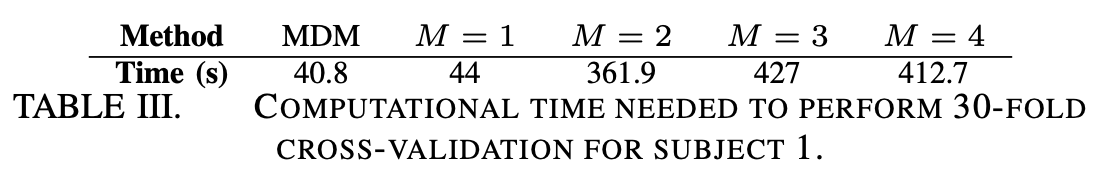
\includegraphics[width=0.8\linewidth]{figs/table-03.png}}
  \vspace{1em}
\end{center}

A tabela acima mostra o tempo de processamento em segundos de cada um dos
classificadores avaliados através do processo de validação cruzada com 30
partes considerando apenas um único indivíduo. Vale notar que a integração
de Monte Carlo e a aproximação por splines são feitas offline e, portanto,
sem influência no tempo de processamento de classificação. Pode-se observar que
para $M=1$ (Gaussiana simples), os tempos de processamento dos classificadores
MDM e Bayes são muito próximos. Contudo, incrementando o valor de $M$
(Gaussiana Mista), o tempo de processamento também aumenta.

\begin{center}
  \vspace{1em}
  \frame{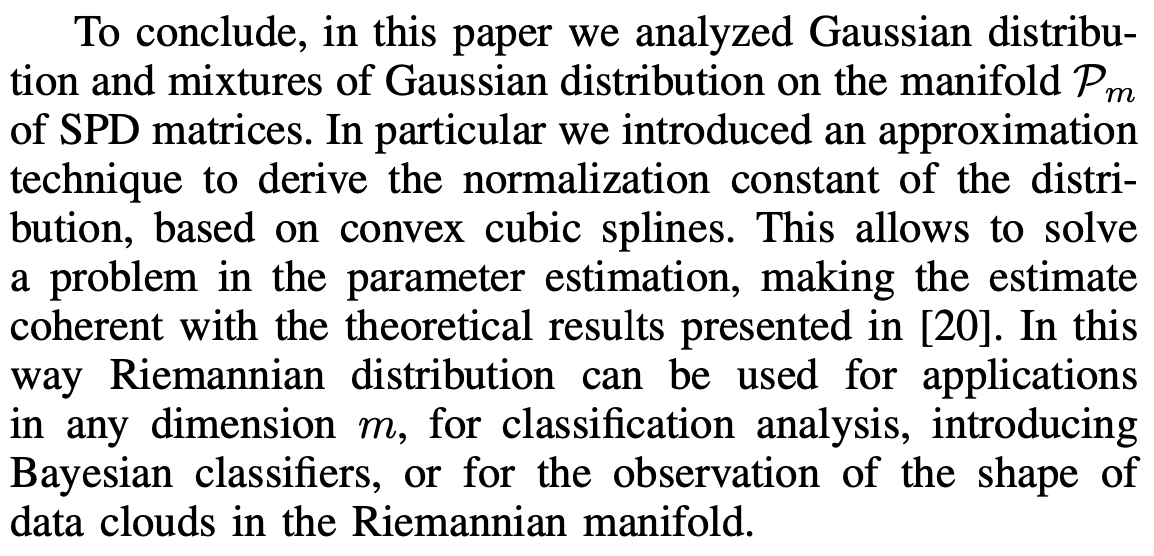
\includegraphics[width=0.8\linewidth]{figs/page-04-paragraph-04.png}}
  \vspace{1em}
\end{center}

Concluindo, neste trabalho técnicas de estimação de parâmetros baseadas em
Geometria Riemanniana foram aplicadas para o problema de classificação no
contexto de EEG\@. Em particular, foi introduzida uma abordagem de aproximação
por splines cúbicos convexos que se mostrou coerente com resultados
consolidados na literatura. Logo, distribuições Riemannianas podem ser
empregadas em qualquer dimensão, para análise de classificação, introduzindo
classificadores Bayesianos, ou observando a estrutura da nuvens de dados na
variedade Riemanniana.  

\bibliographystyle{ieeetr}
\bibliography{refs}
%bib/edge-linking,bib/deformable,bib/medical,bib/graphics,bib/texture,bib/imaging,bib/tracking,bib/shape-papers,bib/bib-header,bib/video,bib/math-books,bib/math,bib/psych-books,bib/metric,bib/edge,bib/leymarie_pami_scaffold,bib/vision-books,bib/vision,bib/nn-search,bib/multidimscaling,bib/psychophysics,bib/indexing,bib/segmentation,bib/image-databases,bib/shape-matching,bib/neuro,bib/skeleton,bib/skeleton2D,bib/aspect-graphs,bib/recognition,bib/surface-networks,bib/ridge,bib/proceedings,bib/perceptual-grouping,bib/continuation,bib/graph-matching-2,bib/cooper}
%\input{paper.bbl}

% Assinaturas:
%\newpage
%\ \\\vspace{7cm}
%\center $\overline{\ \ \ Ricardo\ Fabbri\ \ \ }$
%\ \\\vspace{4cm}
%\center $\overline{\ \ \ Luciano\ da\ Fontoura\ Costa\ \ \ }$
\end{document}
